\documentclass[a4paper, 11pt]{article}
\usepackage{comment} % enables the use of multi-line comments (\ifx \fi) 

\usepackage{fullpage} % changes the margin
\usepackage{longtable}
\usepackage{graphicx}
\usepackage{fancyvrb,xcolor}
\usepackage{listings}
\usepackage{color}
\usepackage[margin=3cm]{geometry}
\usepackage{relsize}
\definecolor{dkgreen}{rgb}{0,0.6,0}
\definecolor{gray}{rgb}{0.5,0.5,0.5}
\definecolor{mauve}{rgb}{0.58,0,0.82}
\definecolor{LightCyan}{rgb}{0.88,1,1}
\usepackage{float}
\usepackage{caption}
\DeclareCaptionFont{white}{\color{white}}
\DeclareCaptionFormat{listing}{\colorbox{gray}{\parbox{\textwidth}{#1#2#3}}}
\captionsetup[lstlisting]{format=listing,labelfont=white,textfont=white}
\newcommand{\bigqm}[1][1]{\text{\larger[#1]{\textbf{?}}}}
\lstset{
  language=Java,
  aboveskip=3mm,
  belowskip=3mm,
  showstringspaces=false,
  columns=flexible,
  basicstyle={\small\ttfamily},
  numbers=none,
  numberstyle=\tiny\color{gray},
  keywordstyle=\color{blue},
  commentstyle=\color{dkgreen},
  stringstyle=\color{mauve},
  breaklines=true,
  breakatwhitespace=true,
  tabsize=3
}
\graphicspath{ {images/} }

\begin{document}
%Header-Make sure you update this information!!!!
\noindent
\large\textbf{Assignment 1} \hfill \textbf{Hussam Hallak} \\
\normalsize CS834, Information Retrieval, Fall 2017\hfill CS Master's Student \\
Old Dominion University, Computer Science Dept \hfill Prof: Dr. Nelson 

\section*{Question 1:}
Exercise 1.1: 

Think up and write down a small number of queries for a web search engine.
Make sure that the queries vary in length (i.e., they are not all one word). Try
to specify exactly what information you are looking for in some of the queries.
Run these queries on two commercial web search engines and compare the top
10 results for each query by doing relevance judgments. Write a report that answers
at least the following questions: What is the precision of the results? What
is the overlap between the results for the two search engines? Is one search engine
clearly better than the other? If so, by how much? How do short queries perform
compared to long queries?

\subsection*{Answer:}
To answer this question, the following queries were tested on both Google and Bing. 

1. Stent

2. Ureteral stent

3. Ureteral stent procedure

4. Do ureteral stents cause pain?

\paragraph{}

I chose these queries because, two weeks ago, I was told by the doctor that I need a ``stent'' to help pass a stone in my kidney. I had no idea what a stent is, so I asked what is a stent? and she explained. Let's pretend that she did not. I want to know what a stent is, the procedure of stenting, the removal of a stent, and whether or not stents cause pain.

\paragraph{1. Stent:}
I ran the first query ``Stent'' and found the following:

A. Google:
Google found about 19,000,000 results. Skipping the ads and looking at the summary given by Google about a stent, I did not see that a stent is related to kidney stones. The summary stated that a stent is a mesh tube that is used to treat narrow or weak arteries. I opened all of the first 10 results returned by Google and found that only the 6th result mentioned something about ureteral stents. Obviously, there are different types of stents for different purposes. I am specifically looking for something related to kidney stones, but I was not specific enough for Google.

Precision is the fraction of retrieved documents that are relevant to the query. In other words, it is the number of correct results divided by the number of all returned results.

$$ 
precision = \frac{|\{relevant\ documents\} \cap \{returned\ documents\}|}{|\{returned\ documents\}|}
$$

$$ 
precision = \frac{1}{10} = 0.1
$$

\pagebreak

\begin{figure}[h]
\caption{Query: Stent, Search Engine: Google}
\centering
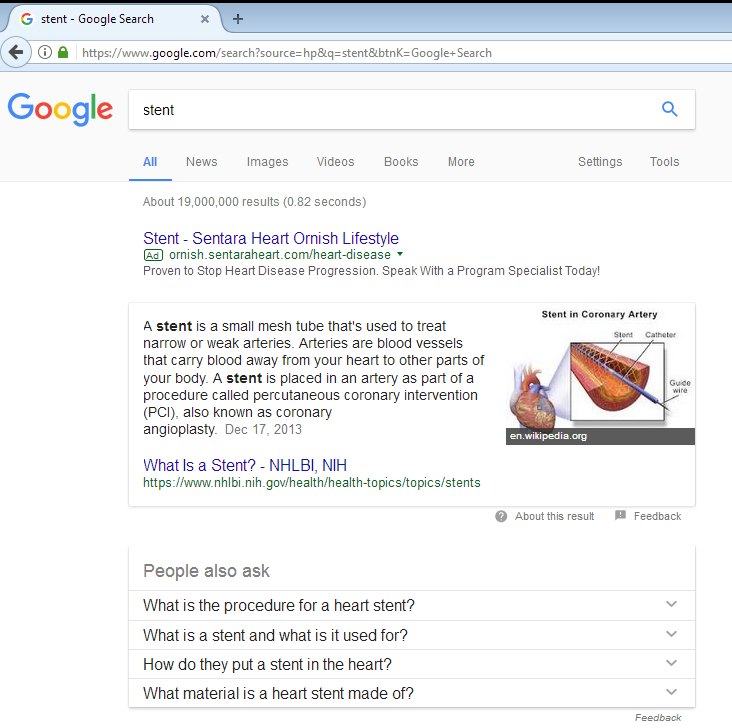
\includegraphics[scale=0.7]{Q1/stent_Google.png}
\end{figure}



B. Bing:
The query returned 23,700,000 results. The summary returned by Bing gave a general definition of a stent. The summary contains exactly what I am looking for ``stents used to allow the flow of urine between kidney and bladder''. This summary, returned by Bing, came from and the document in the 6th result, from wikipedia.org:
https://en.wikipedia.org/wiki/Stent 

Out of the 10 results returned by Bing, Only 3 talked about ureteral stents.

$$ 
precision = \frac{|\{relevant\ documents\} \cap \{returned\ documents\}|}{|\{returned\ documents\}|}
$$

$$ 
precision = \frac{3}{10} = 0.3
$$

\pagebreak

\begin{figure}[h]
\caption{Query: Stent, Search Engine: Bing}
\centering
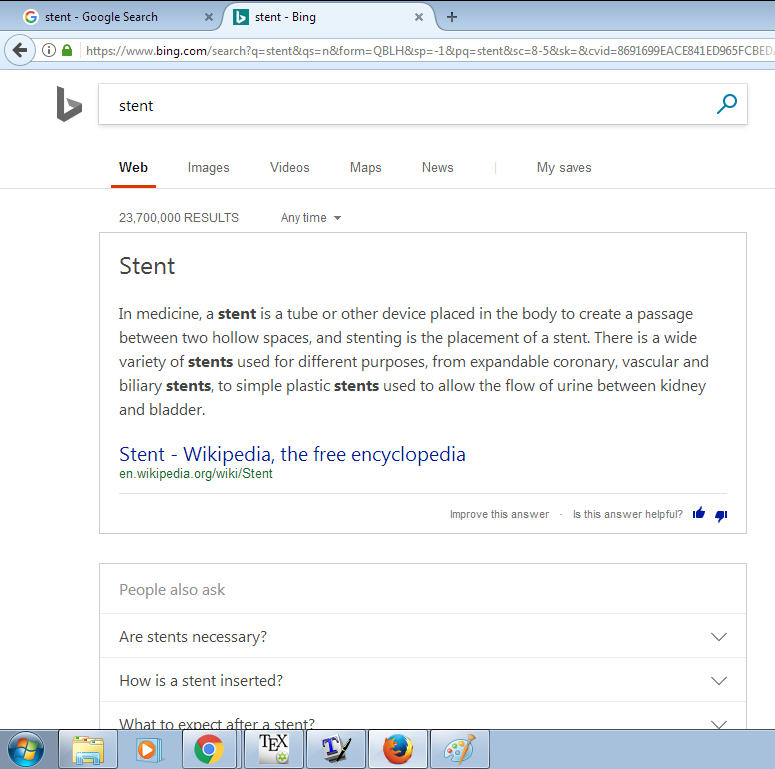
\includegraphics[scale=0.7]{Q1/stent_Bing.png}
\end{figure}

\textbf{Overlap:}
The following table shows the ordered results returned by each search engine: 

\begin{longtable}{ |p{1cm}|p{6cm}|p{6cm}| } 
\hline
Order & Google & Bing \\
 \hline 
 1 & 
 \begin{lstlisting}[breakatwhitespace=〈false)]
http://www.webmd.com/heart-disease/guide/stents-types-and-uses#1
\end{lstlisting} 
&
 \begin{lstlisting}[breakatwhitespace=〈false)]
https://medlineplus.gov/ency/article/002303.htm
\end{lstlisting} 
 \\
 \hline 
 2 & 
\begin{lstlisting}[breakatwhitespace=〈false)] 
https://www.heart.org/idc/groups/heart-public/@wcm/@hcm/documents/downloadable/ucm_300452.pdf
\end{lstlisting}
&
 \begin{lstlisting}[breakatwhitespace=〈false)]
https://en.wikipedia.org/wiki/Coronary_stent
\end{lstlisting} 
  \\ 
 \hline 
 3 & 
\begin{lstlisting}[breakatwhitespace=〈false)]  
https://www.healthline.com/health/stent
 \end{lstlisting}
 &
 \begin{lstlisting}[breakatwhitespace=〈false)]
http://secondscount.org/treatments/treatments-detail?cid=7709f984-f6a5-44bb-8c2f-d7114c5b4c0b
\end{lstlisting} 
 \\
 \hline 
 4 & 
 \begin{lstlisting}[breakatwhitespace=〈false)]
https://www.nhlbi.nih.gov/health/health-topics/topics/stents/
\end{lstlisting}
&
 \begin{lstlisting}[breakatwhitespace=〈false)]
https://www.nhlbi.nih.gov/health/health-topics/topics/stents/
\end{lstlisting} 
\\ 
 \hline
 5 & 
 \begin{lstlisting}[breakatwhitespace=〈false)] 
https://www.nhlbi.nih.gov/health/health-topics/topics/stents/after
  \end{lstlisting}
  &
 \begin{lstlisting}[breakatwhitespace=〈false)]
http://www.webmd.com/heart-disease/guide/stents-types-and-uses
\end{lstlisting} 
 \\
 \hline 
 6 &  
 \begin{lstlisting}[breakatwhitespace=〈false)] 
https://en.wikipedia.org/wiki/Stent
 \end{lstlisting}
 &
 \begin{lstlisting}[breakatwhitespace=〈false)]
https://www.healthline.com/health/stent
\end{lstlisting} 
 \\ 
 \hline 
 7 & 
 \begin{lstlisting}[breakatwhitespace=〈false)]
https://www.nhlbi.nih.gov/health/health-topics/topics/stents/risks
  \end{lstlisting}
  &
 \begin{lstlisting}[breakatwhitespace=〈false)]
http://www.mayoclinic.org/tests-procedures/coronary-angioplasty/home/ovc-20241582
\end{lstlisting} 
  \\
 \hline 
 8 & 
 \begin{lstlisting}[breakatwhitespace=〈false)] 
https://myheart.net/articles/stent-save-life/
  \end{lstlisting}
  &
 \begin{lstlisting}[breakatwhitespace=〈false)]
https://en.wikipedia.org/wiki/Stent
\end{lstlisting} 
 \\ 
  \hline 
 9 & 
\begin{lstlisting}[breakatwhitespace=〈false)] 
http://www.livemint.com/Industry/HMU54RjTrKBHQKPj4QSv0O/Boston-Scientific-may-withdraw-its-highend-stent-Synergy.html
\end{lstlisting}
&
 \begin{lstlisting}[breakatwhitespace=〈false)]
http://medical-dictionary.thefreedictionary.com/stent
\end{lstlisting} 
\\
 \hline 
 10 &  
\begin{lstlisting}[breakatwhitespace=〈false)] 
https://medlineplus.gov/ency/article/002303.htm
\end{lstlisting}
&
 \begin{lstlisting}[breakatwhitespace=〈false)]
https://www.heart.org/idc/groups/heart-public/@wcm/@hcm/documents/downloadable/ucm_300452.pdf
\end{lstlisting} 
\\
 \hline
\end{longtable}

From the table, it is clear that the overlap between the results for the two search engines is six results out of 10 or 60\%.

$$
G_1 \equiv B_5
$$
$$
G_2 \equiv B_{10}
$$
$$
G_3 \equiv B_6
$$
$$
G_4 \equiv B_4
$$
$$
G_6 \equiv B_8
$$
$$
G_{10} \equiv B_1
$$


Where:

$G_i$ denotes the $i$th result returned by Google.

$B_j$ denotes the $j$th result returned by Bing.
 

\paragraph{2. Ureteral Stent:}
 
I ran the query ``Ureteral Stent'' in the same manners as the first query and found the following results:

A. Google:
About 281,000 results are returned by Google.
All of the first 10 results returned by Google, obviously, were related to ureteral stents. Only one of the links did not allow me to read the entire article until I sign up and login to the website, which I did not. I will consider this result not to be a good one because Google returned a result for which the representation of the resource was not retrievable without being a member of the website. All of the remaining 9 results contained information about the procedure, side effects, etc.

$$ 
precision = \frac{9}{10} = 0.9
$$

\pagebreak

\begin{figure}[h]
\caption{Query: Ureteral Stent, Search Engine: Google}
\centering
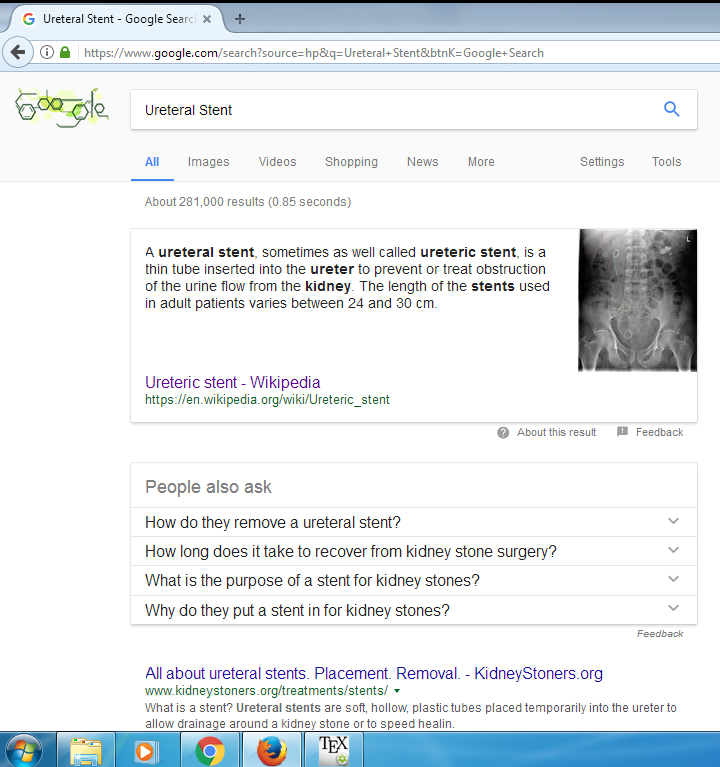
\includegraphics[scale=0.7]{Q1/ureteral_stent_Google.png}
\end{figure}



\pagebreak

B. Bing:

The query returned 2,060,000 result. 8 out of the first 10 retrieved documents contained almost everything I needed to know about ureteral stents. One document listed the types/shapes of ureteral stents, but no other information. One document briefly explained what a ureteral stent is, but did not provide any information about the procedure, complications, side effects, etc.  

$$ 
precision = \frac{8}{10} = 0.8
$$

\begin{figure}[h]
\caption{Query: Ureteral Stent, Search Engine: Bing}
\centering
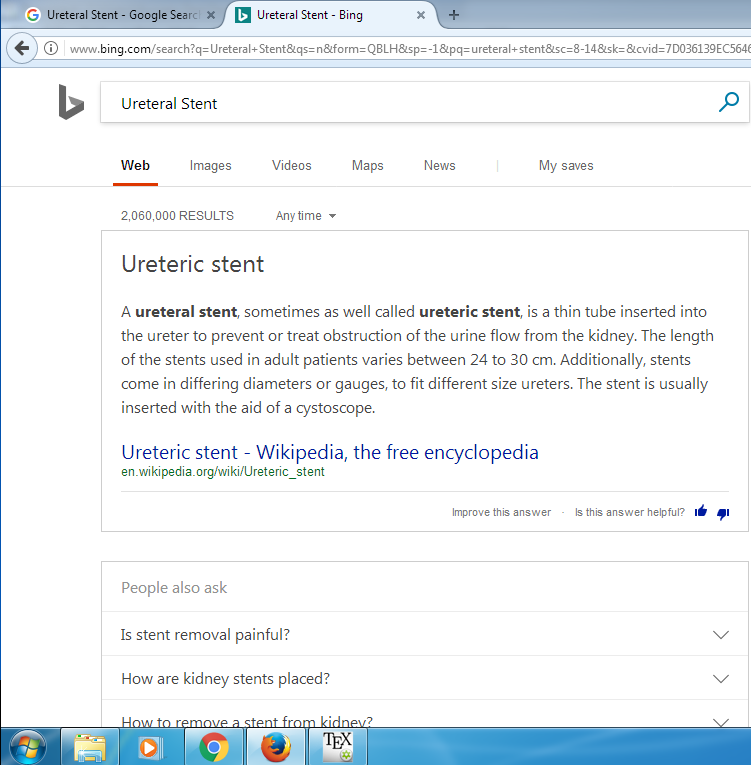
\includegraphics[scale=0.7]{Q1/ureteral_stent_Bing.png}
\end{figure}

\textbf{Overlap:}
The overlap between the results for Google and Bing is 5 out of 10 or 50\%. 

\paragraph{3. Ureteral Stent Procedure:}


Similarly, I ran the query ``Ureteral Stent Procedure''  and found the following results:

A. Google: About 153,000 results are returned by Google. One of the links did not allow me to read the entire article until I sign up and login to the website; the same link was returned running the previous query. One link in the results did not have enough information about the procedure itself, but it had good information about the recovery, diet, etc. All of the remaining 8 results contained information about the procedure, side effects, etc.

$$ 
precision = \frac{8}{10} = 0.8
$$

B. Bing: The query returned 3,330,000 results. 8 out of the first 10 retrieved documents contained enough information about ureteral stent procedure. One document was about stenting pets dogs and cats. One document briefly explained what a ureteral stent is, but did not include the procedure.  

$$ 
precision = \frac{8}{10} = 0.8
$$


\textbf{Overlap:}
The overlap between the results for Google and Bing is 5 out of 10 or 50\%. 

\paragraph{4. Do ureteral stents cause pain?:}

Finally, I ran the query ``Do ureteral stents cause pain?''  and found the following results:

A. Google: About 908,000 results are returned by Google. All of the 10 results had useful information about the pain and ways to manage it.

$$ 
precision = \frac{10}{10} = 1.0
$$

B. Bing: The query returned 163,000,000 results. 8 out of the first 10 retrieved documents contained enough information about the pain associated with ureteral stent procedure and how to manage it. One document had questions from patients answered by doctors, but there was not any questions about the pain. One document briefly explained what a ureteral stent is, but did not include information about the pain.  

$$ 
precision = \frac{8}{10} = 0.8
$$

\textbf{Overlap:}
The overlap between the results for Google and Bing is 6 out of 10 or 60\%. 

\subsection*{Conclusion:}

Bing did a better job on the single word query I ran, while Google got better as the query got longer and more specific.

Average Precision for Google is:

$$ 
precision_{AVG} = \frac{0.1 + 0.9 + 0.8 + 1.0}{4} = 0.7
$$


Average Precision for Bing is:

$$ 
precision_{AVG} = \frac{0.3 + 0.8 + 0.8 + 0.8}{4} = 0.675
$$

The average precision for Google is slightly higher than it is for Bing.

The average overlap between the results for Google and Bing is 55\%:

$$ 
Overlap_{AVG} = \frac{0.6 + 0.5 + 0.5 + 0.6}{4} = 0.55
$$
 
\section*{Question 2:}
Exercise 1.2: Site search is another common application of search engines. In this case,
search is restricted to the web pages at a given website. Compare site search to
web search, vertical search, and enterprise search.

\section*{Answer:}

Site Search: Searching is restricted to the web pages at a given website.

Web Search: Searching all web pages that exist on the web.

Site search engines are applications usually developed by companies that create the websites in order to offer users the ability to search for something within a particular website. For example, if I want to buy a lawn mower, I can go to Home Depot website and type ``lawn mower'' in their search box and click ``SEARCH''. For simplicity, let's assume that Home Depot has a static HTML website and that their search engine greps for the search query in all HTML documents within the website repository. The returned results are all pages that exist on Home Depot website. In this case, no crawling or indexing is needed.

I am sure that Home Depot's website uses a database to store their products information, and that search is performed using SQL queries matching search terms with keywords for each product stored in the database. I just used the example in case of static HTML website as a simplification.

Even if crawling and indexing is implemented in a site search engine, The crawling and indexing is faster and the returned documents are fresher because the crawler and the indexer do not have to crawl and index a massive amount of documents like a web search engine does.

Site search not only ensures the freshness of the returned documents, it also does not have to worry about spam documents like a web search engine does because the site administrator has full control over the website repository. Unless the web-hosting server is compromised, site search should not return spam documents.

A vertical search engine focuses on a specific segment of the web. It is a specialty or topical search engine. The vertical content area could be based on topicality, media type, or genre of content like shopping, images, videos, scholarly literature, etc. For example, Google Shopping is a vertical search engine. Web search engines crawl and index a massive amount of pages on the web. On the other hand, vertical search engines typically use focused crawlers which crawl and index only relevant web pages to a pre-defined topic, media type, etc.

Vertical search has several advantages over web search. Some of which include greater precision because the content crawled and indexed is limited to a certain topic or media type, etc.

Enterprise search is very similar to site search where the domain of focus is the enterprise, such as a company, group of companies, government, or other organizations. Enterprise search makes the content from multiple enterprise-type sources searchable to a defined audience. Examples of Enterprise search include search provided to city employees for a name and address of a property owner, search in medical records saved on Sentara servers  that is provided to doctors and nurses that work for Sentara, etc.

Unlike a web search engine, an enterprise search engine has a much smaller document collection to crawl and index which makes it better in terms of the time needed for crawling and indexing as well as the freshness of the results.

\section*{Question 3:}
Exercise 1.4: List five web services or sites that you use that appear to use search, not including
web search engines. Describe the role of search for that service. Also describe
whether the search is based on a database or grep style of matching, or if the search
is using some type of ranking.

\section*{Answer:}

\textbf{1. ebay.com:}
Ebay is an e-commerce corporation, facilitating online consumer-to-consumer and business-to-consumer sales. The role of search for the service is making the products listed by sellers on ebay.com searchable to buyers. I use it to buy all kind of things. Let's say I wanted to buy a miter saw. I go to ebay.com, type miter saw in the search box, click search, and finally sort by price+shipping low-to-high. Ebay uses Oracle database, so the search is based on a database.

\textbf{2. amazon.com:}
Amazon is an e-commerce and cloud computing company. Amazon is the largest Internet-based retailer. The role of search for the service is the same as Ebay. Amazon uses NoSQL database called DynamoDB. The search is based on a database.

\textbf{3. norfolk.craigslist.org:}
Craigslist is a classified advertisements website and discussion forum. I mostly use it to buy vehicles, various items for my house, used tools, etc. The role of the search is the same as Ebay and Amazon. Craigslist uses a variety of data storage technologies, both SQL (MySQL) and NoSQL (Redis, MongoDB, memcached, etc). The search is based on a database.

\textbf{4. youtube.com:}
Youtube is a video sharing website. The role of the search for the service is making videos hosted on Youtube searchable. Youtube provides videos related to the search query. It uses MySQL database, and the search is based on a database.

\textbf{5. facebook.com:}
Facebook is an online social media and social networking service. The role of the search for the service is making personal profiles, posts, groups, and pages searchable for Facebook users. I use it to find relatives and old friends that I lost contact with due to my moving out of Syria in 2003 before Facebook was launched. Facebook uses MySQL database and the search is based on a database.


\section*{Question 4:}
Exercise 3.8: Suppose that, in an effort to crawl web pages faster, you set up two crawling
machines with different starting seed URLs. Is this an effective strategy for
distributed crawling? Why or why not?

\subsection*{Answer:}
Assuming that the number of machines is fixed. Yes! This is an effective strategy for distributed crawling because otherwise, if we set up both crawling machines with the same starting seed URLs, the chance that both crawlers end up crawling the same pages is large, not only because the starting point is identical, but also because most links on a page lead to pages that are related to it. The likelihood of both crawlers crawling the same pages will decrease if we set them up with different starting seed URLs. The original Google paper stated that Google has a fast distributed crawling system where a single URLserver serves lists of URLs to a number of crawlers (They ran 3). I assume that the URLserver is not serving the same URLs to all 3 crawlers, because if that was the case, there will be no point in adding 2 or more crawlers. I included the bowtie graph I had from CS532 that I took last semester to demonstrate my argument. Please ignore the bowtie itself and focus on the nodes and edges between them. Let's assume that the starting node for both crawlers is P. It is clear that the node N will not be crawled because there is no path from P to N. On the other hand, if we set two different starting points M and P for the first and second crawler respectively, the first crawler will crawl the node N as well as all other nodes crawled by the second crawler.

\begin{figure}[h]
\caption{Bowtie}
\centering
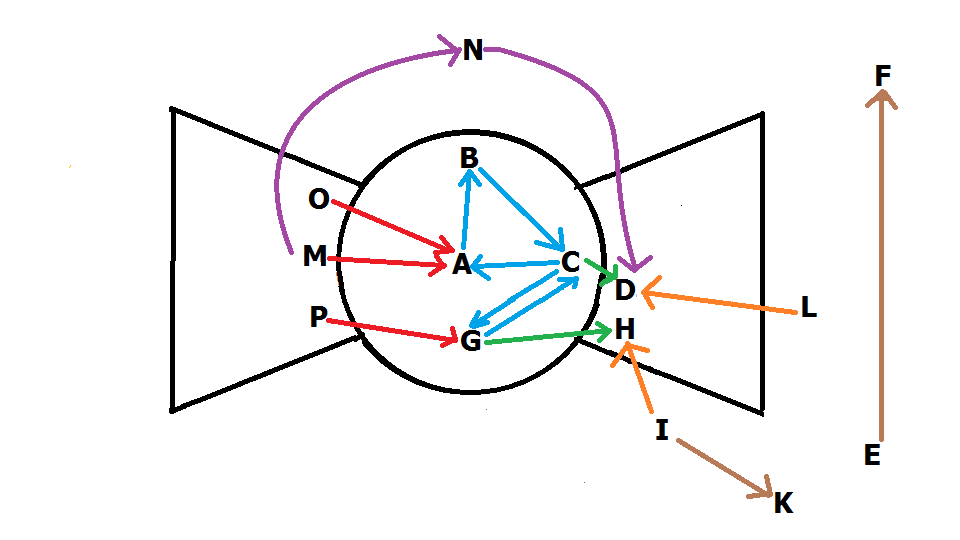
\includegraphics[scale=0.5]{Q4/bowtie.png}
\end{figure}

\section*{Question 5:}
Exercise 3.9: Write a simple single-threaded web crawler. Starting from a single input URL (perhaps a professor’s web page), the crawler should download a page and then wait at least five seconds before downloading the next page. Your program should find other pages to crawl by parsing link tags found in previously crawled documents.

\subsection*{Answer:}
I wrote a simple crawler in python to answer the question. The program expects the user to use two command line arguments as input. The first argument is the seed url and the second one is the number of pages the user wants to crawl and download. Note that the program does not ask or check for the desired crawling depth. The crawler stops crawling when crawling and downloading the entered number of pages is finished.

\textbf{Approach:}
The approach is simple. I summarized it in the following steps:

1. Find the final destination of the seed url.

2. Initialize three sets, arrays with unique elements. They store links to crawl, found links, and crawled links.

3. While there are still links to crawl and the number of desired pages is not reached, repeat the following steps:

a. Pop a url from links\_to\_crawl and pass it to the function crawl to download its content, crawl it, and return the links found in it.

b. Add the crawled link to crawled\_links so it doesn't get crawled again.

c. If the newly returned links are not in found\_links, print them on the screen and add them to found\_links.

d. If the newly returned links are not in crawled\_links, add them to links\_to\_crawl so they can be crawled in the following iterations. 

e. Wait 5 seconds before you crawl and download another page.

\paragraph{}

There are two functions implemented in the program:

1. isAbsolute(url):
This function checks if the passed url, extracted from href attribute in ``a'' tags, is a full or relative link

(e.g., /folder/index.html instead of https://example.com/folder/index.html)

2. crawl(url):
The role of this function is to:

a. Strip the url passed as an argument.

b. Hash the url to use it as a file name for the file that will store the content of the page.

c. Open the url and parse its content using BeautifulSoup and extract all links found in the page and save them to children\_links.

d. Convert relative paths in children\_links to full urls.

e. Iterate through all children links. If they lead to an html page and they return 200 as a status code, save them to the set links\_to\_return. Otherwise print an error message along with the status code for child link.

f. Return the set links\_to\_return.

\textbf{Note:} Simple error handling was used. User input is expected to be well-formatted.

This is the complete code for the program crawler.py:


\lstinputlisting[language=Python, breakatwhitespace=〈false), label=The content of crawler.py, caption= The content of crawler.py]{Q5/crawler.py}

I ran the crawler on Dr. Nelson's web page and passed 10 ``ten pages'' as the number of pages I want to be downloaded.

This is a screen shot of running the crawler:

\begin{figure}[h]
\caption{Running crawler.py}
\centering
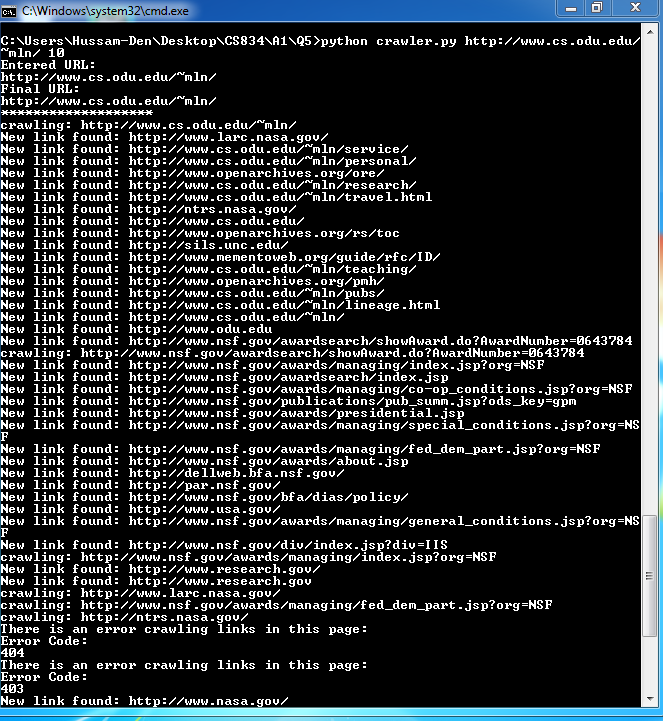
\includegraphics[scale=0.7]{Q5/crawler.png}
\end{figure}

\pagebreak

This is a screen shot of the 10 HTML files downloaded from crawled pages:

\begin{figure}[h]
\caption{Pages downloaded by crawler.py}
\centering
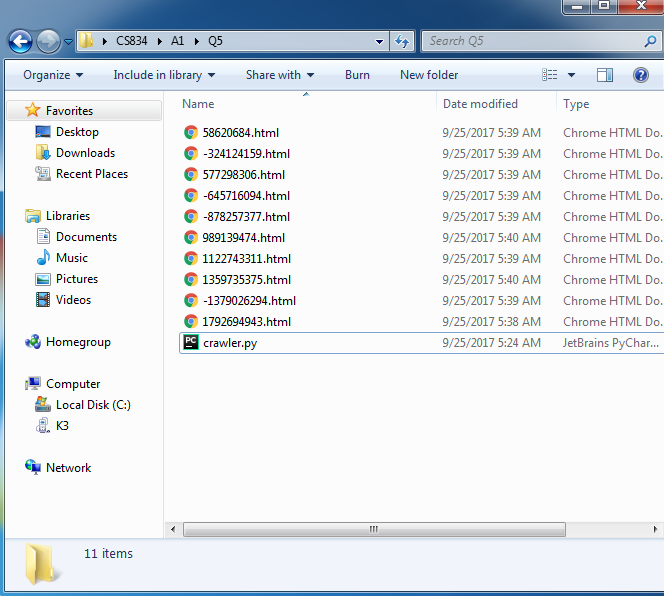
\includegraphics[scale=0.7]{Q5/files.png}
\end{figure}

\begin{thebibliography}{9}

\bibitem{} 
Stackoverflow. https://stackoverflow.com/questions/tagged/python.

\bibitem{} 
Sergey Brin and Larry Page. Google search engine. http://google.stanford.edu.

\bibitem{}
http://www.dba-oracle.com/oracle\_news/news\_ebay\_massive\_oracle.htm

\bibitem{}
https://www.wired.com/2012/01/amazon-dynamodb/

\bibitem{}
https://www.youtube.com/watch?v=a0OvgTfF8Pg

\bibitem{}
http://highscalability.com/blog/2012/3/26/7-years-of-youtube-scalability-lessons-in-30-minutes.html

\bibitem{} http://www.datacenterknowledge.com/data-center-faqs/facebook-data-center-faq-page-2


\end{thebibliography}


\end{document}